\documentclass{article}
\usepackage[utf8]{inputenc}
\usepackage{geometry}
\usepackage{nicefrac}
\usepackage{gensymb}
\usepackage[nowarnings]{xcookybooky}
\usepackage{imakeidx}
\usepackage{float}


\usepackage{hyperref} % this must be the last package that is imported!
\usepackage{bookmark}

\newcommand{\faren}{\degree F }
\renewcommand{\step} % fixing the error with xcookybooky somehow https://tex.stackexchange.com/questions/481698/missing-endcsname-in-package-xcookybooky-texlive
{%
 \stepcounter{step}%shouldn't be in the argument of lettrine
    \lettrine
    [%
        lines=2,
        lhang=0,          % space into margin, value between 0 and 1
        loversize=0.15,   % enlarges the height of the capital
        slope=0em,
        findent=1em,      % gap between capital and intended text
        nindent=0em       % shifts all intended lines, begining with the second line
    ]{\thestep}{}%
}
\geometry{
 letterpaper,
 left=1in,
 top=1in,
 }

\title{Quarantine Cooking}
\author{Drew McNutt and Monica Dayao}
\date{April 2020 (last updated \today)}
\makeindex[intoc]

\begin{document}

\maketitle
\tableofcontents
\newpage
\section{Introduction}
Welcome to our cookbook. It's simply a compilation of recipes we have enjoyed over the past couple of years. Most recipes are vegetarian (because we are). Recipes have been found from all over the internet and from friends and family. If the section headings aren't what you are looking for, we would recommend looking in the index. We have tagged most recipes with relevant tags so you can find exactly what you want.


\begin{center}
    \huge Enjoy!
\end{center}{}

\newpage
\section{Breakfast}
\begin{recipe}[source=Isaac Spiegel]{Shakshuka}
\index{Cast Iron}\index{Mediterranean}\index{Israeli}\index{Kosher!Milk}
\ingredients[11]{%
\unit[4-5]{tbsp} & olive oil \\
1 & pepper \\
1 & onion \\
1 & can of crushed tomatoes \\
\unit[1-2]{tsp} & paprika \\
\unit[1-2]{tsp} & cumin \\
\unit[1-2]{tsp} & cayenne \\
\unit[1-2]{tsp} & salt \\
1 & feta block \\
\unit[2]{cloves} & garlic \\
4-6 & eggs \\
Some & pepper \\
}
\preparation{%
\step Preheat oven to about 350\faren. Heat 4-5 tablespoons of oil in a large cast iron pan.
\step Chop the onions and peppers and saute in the hot pan until dark brown.
\step Add the garlic, paprika, cumin, cayenne and salt. Saute for about 5 more minutes.
\step Add the crushed tomatoes and let simmer. The length of this simmer is up to you, a longer simmer means a chunkier final product.
\step Dig out a small hole, go all the way to the bottom of the pan and crack an egg into it. Repeat this 3-5 more times.
\step Crack some fresh pepper on top of the eggs. Crumble the entire block of feta, covering the entire pan with cheese. 
\step Put in the oven and cook until the eggs have set. Should take about 10 minutes, but keep an eye on them so you can get nice runny eggs.
}
\end{recipe}


\newpage
\begin{recipe}[source=\href{https://www.marthastewart.com/338185/basic-pancakes}{Martha Stewart}]{Pancakes}
	\index{Easy}\index{Cast Iron}\index{American}
	\ingredients[6]{%
		\unit[130]{g} & flour \\
		\unit[2]{tbsp} & sugar \\
		\unit[2]{tsp} & baking powder \\
		\unit[\nicefrac{1}{2}]{tsp} & salt \\
		\unit[1]{cup} & milk \\
		\unit[2]{tbsp} & vegetable oil \\
		1 & egg \\
	}
	\preparation{%
		\step Preheat oven to 200\faren and place a cookie sheet in the oven so that you can keep the pancakes warm after you make them.
		\step In a small bowl, combine the flour, sugar, baking powder, and salt.
		\step In another small bowl, combine the milk, oil (or melted butter), and egg. Add the dry ingredients to the wet ingredients and whisk until just moistened, small lumps are perfectly fine.
		\step Heat a large skillet over medium heat. Coat the pan with a thin layer of oil.
		\step Spoon about \nicefrac{1}{4} cup of the batter onto the skillet. Cover with the toppings of your choice (e.g. chocolate chips, banana slices, blueberries, etc. )
		\step Cook until surface of pancakes are covered in bubbles, then flip with a spatula. Cook until browned. Each side should take 1-2 minutes.
		\step Throw onto the baking sheet in the oven to keep warm after cooking.
	}
\end{recipe}


\newpage
\input{Breakfast/tortang_talong}

\newpage
\begin{recipe}[source=\url{https://thefoodietakesflight.com/vegan-mushroom-tocino/}]{Mushroom Tocino}
        \index{Filipino}\index{Mushrooms}
        \ingredients[10]{%
                \multicolumn{2}{l}{\large Marinade}\\ [0.2cm]
                \unit[3-4]{tbsp} & brown sugar \\
                \unit[2]{cloves} & garlic \\
                \unit[1]{tbsp} & soy sauce \\
                \unit[1]{tbsp} & vinegar \\
                \unit[3]{tbsp} & pineapple juice \\
                \unit[\nicefrac{1}{2}]{tsp} & annato or atsuete powder (optional) \\
                                            & ground black pepper \\
                \multicolumn{2}{l}{\large Tocino}\\ [0.2cm]
                \unit[250]{g} & fresh oyster mushrooms \\
                \unit[1]{tbsp} & neutral oil \\
                pinch & salt \\
        }
        \preparation{%
                \step Mix together all the ingredients for the marinade in a large bowl until the sugar has dissolved. Feel free to adjust to your desired sweetness and acidity.
                \step Mix the mushrooms in the marinate to completely soak and coat in the sauce. Leave the mushrooms to sit for at least 15 minutes. You can also refrigerate these to marinate overnight.
                \step Note: if cooking some sinangag (garlic fried rice), I suggest to cook this in the same pan before cooking the mushrooms. 
                \step Heat a large pan over medium high heat. Once hot, add in the oil. Place the mushrooms along with the marinating liquid into the pan. Leave the mushrooms to cook over medium to medium high heat until the liquid slowly evaporates. The sugars will slowly cook down and start to beautifully coat the mushrooms.
                \step You can leave the mushrooms untouched for 3-4 minutes to lightly brown and char at the bottom before mixing to cook the remaining sides. You can add a pinch of salt to season the mushrooms, if you’d like.
                \step Continue to cook the mushrooms down until all the sauce has been absorbed and the mushrooms have turned shiny and have a thin glaze-like coating from the sugars that have cooked down.
                \step Serve your tocino with some sinangag (garlic fried rice), suka’t sili (vinegar with some chiles and onions), and kamatis (tomatoes) for the perfect hearty Filipino breakfast that can also be enjoyed any time of the day. Enjoy!
        }
        \hint{
                This recipe can be adapted to use other types of mushrooms, seiten, or tofu!
        }
\end{recipe}


\newpage
\section{Curries}
\begin{recipe}[
	]{Baingan Masala (Spicy Eggplant Curry)}\index{Indian}\index{Spicy}\index{Eggplant}
\ingredients[20]{%
	plenty of & oil\\
	\unit[\nicefrac{1}{4}]{tsp} & garlic powder \\
	\unit[\nicefrac{1}{4}]{tsp} & onion powder \\
	4 & green chilies \\
	\unit[2]{tbsp} (\unit[22]{g}) & ginger \\
	\unit[\nicefrac{3}{4}]{tsp} & turmeric powder \\
	5 & tomatoes \\
	\unit[3]{tsp} & coriander powder \\
	\unit[3]{tsp} & kashmiri chili powder\\
	\unit[3]{tbsps} & shredded coconut \\
	\unit[2]{tsp} (divided)& salt \\
	\unit[800]{g} & eggplant \\
	\unit[1\nicefrac{1}{2}]{tsp} & cumin seeds\\
	\unit[1]{tsp} & mustard seeds\\
	3 & bay leaves \\
	1 & cinnamon stick \\
	\unit[2]{cups} & water \\
	\unit[\nicefrac{3}{4}]{tsp} & garam masala \\
	\unit[4-5]{sprigs} & cilantro (coriander) leaves \\
}
\preparation{
	\step Heat 5-7 tablespoons oil in a large pan on medium-high heat.
	\step Chop up the ginger into small pieces. Cut the tomatoes into large pieces.
	\step Add the garlic powder, onion powder, green chilies, chopped ginger, turmeric, and tomatoes to the pan. Mix well and saute for 1 minute.
	\step Add the coriander powder, chili powder, and shredded coconut. Mix in and saute for 1 minute. Put heat on low and cover for 2 minutes.
	\step Add 1 teaspoon of salt and mix well. Remove the pan from the stove and set aside to cool.Once the mixture is cool enough, blend it into a smooth paste.
	\step Cut the eggplant up into large cubes (or cut Xs into the bottoms of small eggplants all the way to the stem).
	\step Heat deep frying oil on medium to high heat. (Also now is a good time to pressure cook some rice)
	\step Gently add the eggplant to boil (Don't splash the oil!).
	\step Deep fry for 3-4 minutes, or until soft, stirring after 1 minute and flipping occasionally for even cooking. Set aside on paper towels to drain oil. 
	\step Heat 4-5 tablespoons oil on high heat. Add the cumins seeds, mustard seeds, bay leaves, and cinnamon stick. Saute untill fragrant (the mustard seeds popping is normal, but don't let it go too crazy). 
	\step Add the blended paste (be careful it will probably splash a bit), and add about 1 teaspoon salt, or to taste and mix well.
	\step Stir until the mixture begins to bubble. Lower the heat and cover. Let simmer for about 6 minutes.
	\step Add the water to the blender (gotta clean out all of the yummy paste) to rinse it off.
	\step Add the blender water to the stove and mix well. Bring the mixture to a boil. Lower the heat a bit and let simmer for 3 minutes with the lid on.
	\step Add the fried eggplants and mix well. Set the heat to medium, cover with a lid and cook for 5 minutes.
	\step Add the garam masala and cilantro leaves, mix well. Enjoy!
}
\suggestion{
	\begin{itemize}
		\item You can add 4 dried kashmiri chilies at the beginning if you want extra heat, but the 4 green chilies are plenty
		\item Instead of the 5 tomatoes you can use 600 grams crushed tomatoes. Then you can avoid cutting up the tomatoes!
	\end{itemize}
}
\end{recipe}


\newpage
\begin{recipe}[source=\url{https://www.cookwithmanali.com/sarson-ka-saag/},portion=\portion{4-6}]{Sarson ka Saag Paneer}
        \index{Indian}\index{Paneer}
\ingredients[28]{
        \multicolumn{2}{l}{\large To Pressure Cook}\\[0.2cm]
        \unit[250]{g} & mustard greens \\
        \unit[250]{g} & mixed greens such as spinach \\
        1 & medium onion, chopped\\
        5-6 & garlic cloves, chopped \\
        \unit[1]{in} & ginger, chopped\\
        2 & green chilies (or to taste), chopped \\
        \unit[3]{in} & white radish, chopped \\
        \unit[\nicefrac{1}{2}]{tsp} & red chili powder \\
        \unit[1]{tsp} & salt \\
        \unit[1.5]{cups} & water\\
                         & \\
        \unit[2]{tbsp} & maize flour \\
                       & \\
        \multicolumn{2}{l}{\large Tempering/Tadka} \\[0.2cm]
        \unit[2]{tbsp} & ghee \\
        \unit[\nicefrac{1}{4}]{tsp} & hing/asafetida \\
        3-4 & garlic cloves, chopped \\
        1 & medium onion, chopped \\
        2 & dried red chilies \\
        \unit[\nicefrac{1}{2}]{tsp} & coriander powder \\
        \unit[\nicefrac{1}{2}]{tsp} & garam masala \\
                                    & \\
        \multicolumn{2}{l}{\large Paneer} \\[0.2cm]
        \unit[2]{blocks} & paneer, cut into half in cubes \\
        \unit[2]{tbsp} & ghee or oil
}
\preparation{
\step Add the chopped onion, garlic, ginger and green chilies to the pressure cooker on `saute' mode. Saute for a few minutes until parts of the onion turn brown. Wash and chop the greens then add them to the pressure cooker.
\step Add tomatoes and white radish. Then add the red chili powder and salt. Add 1.5 cups water and stir.
\step Cook on high pressure for 5 mins and then let the pressure release naturally. Alternatively, you can also cook everything on a stove top for 20-25 minutes until soft.
\step Open the instant pot and then use an immersion blender to puree the saag. If you don't have an immersion blender, wait for it cool down a bit and then puree using your regular blender.
\step Blend to a coarse paste. You can make it as smooth/coarse as you like.
\step Transfer saag to another pot on stove top over medium-low heat. Add 2 tablespoons of maize flour to the saag and mix, this helps in thickening the saag. Regular flour or cornstarch can also be used if you don't have maize flour.
\step Set heat to low and let the saag simmer for 20 to 25 minutes on low heat. It will thicken as it simmers.
\step In the meantime, cut up your paneer into half inch cubes and pan fry with oil or ghee until they are brown on each side.
\step For the final tadka, heat a small pan on medium heat. Once the pan is hot add ghee to it and then add hing and chopped garlic cloves. Saute for few seconds and then add the chopped onion and dried red chilies.
\step Cook until the onions and garlic turn light golden brown. Add the coriander powder and garam masala and mix.
\step Transfer the tadka/tempering to the saag and mix. Then transfer the paneer into the saag and mix.
\step Serve sarson ka saag with makki roti, sliced onion, jaggery and white butter! 
}
\hint{ 
        If you have an air fryer, you can use it to fry up the paneer cubes.
}
\end{recipe}


\newpage
\section{Side Dishes}
\begin{recipe}{Hummus}
\index{Chickpeas}\index{Vegan}\index{Mediterranean}\index{Israeli}
\ingredients[7]{
    \unit[\nicefrac{1}{4}]{cup} & lemon juice \\
    \unit[\nicefrac{1}{4}]{cup} & tahini \\
    \unit[1]{clove} & garlic \\
    \unit[2]{tbsp} & olive oil \\
    \unit[\nicefrac{1}{2}]{tsp} & cumin \\
    \unit[1]{tsp} & salt \\
    \unit[250]{g} & cooked chickpeas \\
}
\preparation{%
    \step In a food processor combine the tahini and lemon juice. Process for 1 minute, scrape down the sides of the bowl and process for 30 more seconds.
    \step Mince the garlic. Add the olive oil, minced garlic, cumin, and \nicefrac{1}{2} teaspoon of salt to the food processor. 
    \step Process for 30 seconds, scrape down the sides of the bowl and process again for 30 seconds.
    \step Add half of the drained chickpeas and process for 1 minute. 
    \step Scrape down the sides of the bowl and add the remaining chickpeas. Process unitl smooth, 1-2 minutes.
    \step If the hummus is still thick or chunky, add water a tablespoon at a time while the processor is on. Should only require about 2 to 3 tablespoons of water. 
}
\end{recipe}


\newpage
\begin{recipe}[source=\url{https://www.themediterraneandish.com/smoky-eggplant-dip-baba-ganoush/}]{Baba Ganoush}
\index{Eggplant}\index{Vegan}\index{Mediterranean}
\ingredients[]{
1 & large eggplant (or 2-3 small) \\
\unit[2]{tbsp} & tahini \\
1-2 & garlic cloves, chopped \\
\unit[1]{tbsp} & lemon juice \\
to taste & salt and pepper\\
\unit[\nicefrac{1}{4}]{tsp} & crushed red pepper \\
\unit[1]{tsp} & sumac, optional
}
\preparation{%
\step Smoke the eggplant. Turn 1 gas burner on medium or high (will depend on the burner). Using a pair of tongs, turn eggplant every 5 minutes or so until the eggplant is completely tender and it’s skin is charred and crispy (about 15 to 20 minutes.) Don’t worry if the eggplant deflates, it’s supposed to. (You can also do this on a gas or charcoal grill over medium-high heat.) Remove from heat and let the eggplant cool.
\step Once eggplant is cool enough to touch, peel the charred crispy skin off. Discard the stem. Transfer eggplant flesh to a colander; let drain for 3 minutes.
\step Transfer eggplant flesh to the bowl of a food processor. Add tahini paste, yogurt, garlic, lemon juice, salt, pepper, crushed red pepper, and sumac (if using). Give it just a couple of pulses to combine (do not over blend, you want to keep it chunky).
\step Transfer the baba ganoush spread to a small bowl. Cover and refrigerate for an hour (if you don’t have the time, try refrigerating for a few minutes to let the flavors meld and the baba ganoush thicken a bit). Just before serving, top the baba ganoush with a sprinkle of sumac, olive oil, toasted pine nuts, parsley leaves, or anything other Mediterranean spice. Enjoy with a side of warm pita bread or pita chips. 
}
\hint{
If you do not have the means to cook the eggplant over an open flame, you can roast the eggplant in the oven at 425 \faren for about 30-40 min. Cut the eggplant in half and make slits in the skin before roasting.
}
\end{recipe}


\newpage
\begin{recipe}[
	preparationtime={\unit[40]{min}},
	bakingtime={\unit[45]{min}},
	portion=\portion{4-6},
	bakingtemperature={\protect\bakingtemperature{fanoven=\unit[275]{\faren}}},
	source=Mom
	]{Carrot Souffle}\index{Jewish}
\ingredients{%
\unit[1]{lb.} & carrots\\
\unit[4]{oz.} & butter\\
3 & eggs\\
\unit[\nicefrac{1}{2}]{Cup} & sugar\\
\unit[3]{tablespoon}& flour\\
\unit[1]{teaspoon} & baking powder\\
\unit[1]{teaspoon} & vanilla extract\\
to taste & salt \\}

\preparation{
\step Peel carrots and cook in salted water until well done (about 30 minutes). Drain Carrots.
\step Melt Butter. Preheat Oven to 275\faren
\step Put eggs, melted butter, sugar, flour, baking powder, and vanilla in a blender and blend well. Add carrots and blend until the mixture resembles a milk shake. 
\step Pour into a greased 8x8 inch glass dish and bake at 275\faren\,for 45 minutes.
}
\hint{
You can use a food processor instead of a blender.
}
\end{recipe}{}


\newpage
\begin{recipe}[source=\href{https://www.foodnetwork.com/recipes/dave-lieberman/noodle-kugel-recipe-1946564}{Dave Lieberman}]{Noodle Kugel}       
	\index{Jewish}\index{Kosher!Passover}\index{Kosher!Milk}\index{Casserole}
	\ingredients[6]{%
		\unit[\nicefrac{1}{2}]{lbs} & wide egg noodles \\
		\unit[\nicefrac{1}{4}]{cup} & butter \\
		\unit[1]{lb} & cottage cheese \\
		\unit[2]{cups} & sour cream \\
		\unit[\nicefrac{1}{2}]{cup} & sugar \\
		6 & eggs \\
		\unit[1]{tsp} & cinnamon \\
		\unit[1]{can} & crushed pineaple in juice \\
	    }

	    \preparation{%
		\step Heat the oven to 375 \faren.
		\step Boil the noodles in salted water for about 4 minutes or until slightly undercooked (it will cook more in the oven). Strain the noodles.
		\step While the noodles are cooking, melt the butter and drain the pineapple.
		\step Grease a $9\times13$ inch baking dish.
		\step Combine all of the ingredients in a large bowl, then transfer to the baking dish.
		\step Bake for 30-45 minutes or until the top is golden brown.
	    }
\end{recipe}        


\newpage
\begin{recipe}[source=Mom]{Matzo Ball Soup}
\index{Soup}\index{Jewish}\index{Kosher!Passover}
\ingredients{%
\unit[\nicefrac{3}{4}]{Cup} & Matzo Meal\\
2 & Eggs\\
\unit[3]{tablespoons} & Oil\\
& Garlic Salt \\
& Dill \\
& Ginger\\
& Black Pepper\\
}
\preparation{%
\step Mix all of the ingredients. Let rest in refrigerator for at least 30 minutes.
\step Lightly form the mixture into balls (do not roll the balls). The key is to form a ball without making it too dense
\step Boil in Veggie Stock for 30 minutes}
\end{recipe}{}


\newpage
\begin{recipe}[bakingtime={\unit[30]{min}},portion=\portion{4},source=\url{https://thewoksoflife.com/mexican-rice-recipe/}]{Mexican Rice}
\index{Rice}\index{Mexican}
\ingredients[10]{
\unit[1\nicefrac{1}{2}]{tbps} & oil \\
\unit[1\nicefrac{1}{4}]{cups} & uncooked white rice \\
\unit[1\nicefrac{1}{2}]{cups} & low-sodium chicken or vegetable stock \\
\unit[1]{tbsp} & tomato paste \\
\unit[\nicefrac{1}{2}]{tsp} & onion powder \\
\unit[\nicefrac{1}{2}]{tsp} & garlic powder \\
\unit[\nicefrac{1}{2}]{tsp} & cumin \\
\unit[\nicefrac{1}{4}]{tsp} & chili powder \\
\unit[\nicefrac{1}{4}]{tsp} & black pepper \\
\unit[\nicefrac{1}{4}]{tsp} & salt \\
}
\preparation{
\step Heat 1.5 tablespoons of oil in a deep skillet set over medium-high heat. Add the rice and stir constantly until the rice begins to turn golden brown. The toastier your rice, the tastier it will be.
\step Next, add the chicken stock. The mixture will bubble up, and should be followed immediately by the tomato paste or tomato sauce, onion powder, garlic powder, cumin, chili powder, black pepper, and salt.
\step Bring to a boil, stirring the tomato paste to dissolve it if using, and cover with a tight-fitting lid. Immediately turn the heat down to low and set a timer for 20 minutes.
\step You may want to check on moisture levels while the rice is cooking. If it looks like the rice needs more water, add \nicefrac{1}{4} cup at a time or until you think the rice is cooked well.
\step When the rice is done, fluff it with a fork and serve!
}

\hint{
\begin{itemize}
    \item If you don't have tomato paste, you can replace it with \nicefrac{1}{2} cup of plain tomato sauce.
    \item Feel free to add more of the spices than in the recipe. The first time I made this, I accidentally doubled the amounts, and it still turned out great.
\end{itemize}
}
\end{recipe}


\newpage
\begin{recipe}[source=Lucy]{Tomatillo Salsa}
	\index{Mexican}\index{Spicy}\index{Easy}
	\ingredients{%
		4-5 & tomatillos \\
		\unit[1]{clove} & garlic \\
		\nicefrac{1}{4} & onion \\
		1-2 & jalapenos \\
	}
	\preparation{%
		\step Peel and wash the tomatillos.
		\step In a large pot combine the garlic, onion, and tomatillos. Note: you do not have to chop or peel the garlic or onion. Fill with enough water to cover all of the ingredients and bring to a boil.
		\step Simmer the pot until the tomatillos have completely changed color.
		\step Drain all of the water and add all of the solids to a blender
		\step Blend until slightly chunky, then add the jalapenos. If you do not want the salsa to be too spicy you can deseed the jalapenos before adding.
		\step Blend until jalapenos are combined into the chunky green salsa.
	}
\end{recipe}


\newpage
\begin{recipe}{Corn Fritters}
\index{Fried}\index{Corn}
\ingredients[]{%
\unit[190]{g} & flour \\
\unit[2]{cups} & corn \\
\unit[50]{g} & shredded cheddar cheese \\
\unit[15]{g} & chives \\
\unit[1/2]{cup} & milk \\
2 & eggs \\
\unit[1]{tsp} & salt \\
\unit[1]{tsp} & kashmiri chili powder \\
\unit[\nicefrac{1}{2}]{tsp} & onion powder \\
\unit[\nicefrac{1}{2}]{tsp} & garlic powder \\
\unit[\unit[1]{2}]{cup} & oil
}
\preparation{
\step Combine all ingredients (except for the oil) in a large bowl
\step Heat the oil (make sure its enough to coat the entire bottom of the pan) in a skillet on medium heat
\step When the oil is hot, add 2 tablespoons of the mixture to the oil and press down to make flat
\step Flip after about 2 minutes, or until the bottom is sufficiently crispy
\step Fry on the last side for another 2 minutes, then remove from the oil and place on a paper towel lined plate
}
\hint{You can replace the egg with a chia seed egg and the milk with a non-dairy milk
}
\end{recipe}


\newpage
\begin{recipe}[source=\href{https://www.reddit.com/r/theppk/wiki/kitchen/favoriterecipes/seitanogreatness?utm_source=share\&utm\_medium=ios\_app\&utm\_name=iossmf}{Post Punk Kitchen Reddit}]{Seitan}
    \index{Chicken Wings}\index{Sandwich Meat}
	\ingredients{%
		\unit[180]{g} & vital wheat gluten \\
		\unit[\nicefrac{1}{4}]{cup} & nutritional yeast \\
		\unit[1]{tsp} & salt \\
		\unit[2]{tsp} & paprika \\
		\unit[\nicefrac{1}{4}]{tsp} & cinnamon \\
		\unit[\nicefrac{1}{4}]{tsp} & cumin \\
		\unit[1]{tsp} & black pepper \\
		\unit[\nicefrac{1}{8}]{tsp} & cayenne pepper \\
		\unit[1]{tsp} & garlic powder \\
		\unit[\nicefrac{3}{4}]{cup} & cold water \\
		\unit[4]{tbsp} & tomato paste \\
		\unit[2]{tbsp} & olive oil \\
		\unit[1]{tbsp} & soy sauce \\
		\unit[2]{tbsp} & worcestershire sauce \\
	}
	\preparation{%
		\step In a large bowl, combine all of the dry ingredients and mix well.
		\step In a separate medium bowl, combine all of the wet ingredients and mix well.
		\step Add the wet ingredients to the dry and stir until all of the dry material is incorporated.
		\step Turn out the bowl onto a clean surface and knead the dough until you are content.
		\step At this point you can shape the seitan into whatever shape you would like for your specific use (i.e. wings, log, small sausages, etc. )
		\step Preheat oven to 325\faren.
		\step If shaping into a large log, wrap the entire piece of dough with aluminum foil twisting the ends. Bake for 90 minutes and unwrap when done to fully cool.
		\step Alternatively, if making chkn wings then form into many small nuggets on a greased baking sheet. Bake for about 30 minutes, flipping once in the midway through.
	}
\end{recipe}


\newpage
\begin{recipe}[source=\url{https://www.cookwithmanali.com/cilantro-yogurt-chutney/}]{Cilantro Chutney}
\index{Cilantro}\index{Indian}\index{Chutney}
\ingredients[7]{
    \unit[100-120]{g} & cilantro \\
    1 & green chili \\
    \unit[\nicefrac{1}{2}]{inch} & ginger \\
    \unit[\nicefrac{1}{4}]{tsp} & roasted cumin powder \\
    \unit[\nicefrac{1}{8}]{tsp} & chaat masala \\
    pinch & black pepper \\
    \unit[\nicefrac{1}{2}]{tsp} & salt \\
    \unit[2]{tsp} & lemon juice \\
    \unit[\nicefrac{1}{2}]{tsp} & sugar \\
    \unit[\nicefrac{1}{4}]{cup} & yogurt \\
}
\preparation{%
	\step Remove any hard stems or stalks from the cilantro (tender/small ones are okay)
	\step Add all of the ingredients to the blender.
	\step Blend everything together to a smooth consistency. If it is still a bit runny you can add some peanuts to the chutney, 3-4 whole peanuts at a time (you may want to roughly chop them first so they actually get blended).
	\step You can freeze or refridgerate the chutney and use as needed.
}
\end{recipe}


\newpage
\begin{recipe}[source=\url{https://www.cookwithmanali.com/onion-tomato-chutney/}]{Tomato Chutney}
\index{Tomato}\index{Indian}\index{Chutney}
\ingredients[15]{
    \unit[\nicefrac{1}{2}]{tbsp} & oil or ghee \\
    \unit[1.5]{tsp} &  chana dal (split baby chickpeas) \\
    3-4 & garlic cloves \\
    1 & small onion \\
    2-3 & dried red chiles \\
    2 & large tomatoes \\
    \unit[\nicefrac{1}{2}]{tsp} & salt \\
    \unit[\nicefrac{1}{4}]{tsp} & red chili powder \\
                                & \\
    \multicolumn{2}{l}{\large Tempering/Tadka} \\[0.2cm]
    \unit[1]{tsp} & oil or ghee \\
    \unit[\nicefrac{1}{4}]{tsp} & mustard seeds \\
    pinch & hing \\
    6-7 & curry leaves (optional)\\
}
\preparation{%
    \step Heat 1/2 tablespoon of oil in a kadai/pan on medium heat. Once the oil is hot, add the chana dal and cook for around 2-3 minutes or until the dal is golden in color. Remove the dal from pan and set aside.
    \step To the same pan now add garlic, onion and dried red chilies. Increase the amount of red chilies as per your taste. 
    \step Cook for around 3 minutes until the onions are soft. Then add in the tomatoes and salt and stir.
    \step Cook the tomatoes until they are soft and mushy, around 6-7 minutes. Let it cool down a bit and then transfer to a blender along with the roasted chana dal.
    \step Grind to a smooth paste. Add 1/4 teaspoon kashmiri red chili powder while grinding but that's optional. Transfer chutney to a bowl. 
    \step To make the tadka/tempering, heat 1 teaspoon oil in a small pan on medium heat. Once the oil is hot, add the mustard seeds and let them pop. Then add the hing and curry leaves. Saute for a minute until the curry leaves turn little crisp.
    \step Transfer the tempering to the tomato chutney and mix. Enjoy tomato chutney with dosa/idlis or even parathas.
}
\hint{
        You may also add roasted peanuts to this chutney if you'd like.
}
\end{recipe}


\newpage
\begin{recipe}[source=\href{https://thewoksoflife.com/smashed-asian-cucumber-salad/}{The Woks of Life}]{Smashed Cucumber Salad}
\index{Cucumber}\index{Chinese}
\ingredients[12]{
        2-3 & cucumbers (around 600g) \\
        \unit[1]{tsp} & salt \\
        \unit[2\nicefrac{1}{2}]{tsp} & sugar \\
        \unit[2]{tsp} & sesame oil \\
        \unit[3]{tsp} & light soy sauce \\
        \unit[1\nicefrac{1}{2}]{tbsp} & rice vinegar \\
        2-4 & garlic cloves, finely chopped \\
        \unit[2]{tsp} & toasted sesame seeds \\
        small handful & chopped cilantro
}
\preparation{%
        \step Wash the cucumbers and pat them dry with a clean towel. Make the salad dressing by combining the salt, sugar, sesame oil, light soy sauce, and rice vinegar. Stir until the sugar and salt are completely dissolved. Set aside.
        \step On a cutting board, lay a large knife flat against the cucumber, and smash it lightly with your other hand. The cucumber should crack open and smash into four sections. Repeat along its full length. Once the whole cucumber is completely open (usually into 4 long sectional pieces), cut it at a 45-degree angle into bite-sized pieces. 
        \step In a large bowl, mix the cut cucumber with the prepared dressing, garlic and chili oil, and toss it well. Serve, garnished with sesame seeds and cilantro.
}
\end{recipe}


\newpage
\section{Entrees}
\begin{recipe}[source=\url{https://frommybowl.com/buffalo-cauliflower-chickpea-casserole/}]{Buffalo Cauliflower \& Chickpea Casserole}
\index{Cast Iron}\index{Spicy}
\ingredients[6]{%
	\nicefrac{1}{2} & onion \\ 
	\unit[2]{cloves} & garlic \\
	\unit[2]{cups} & vegetable broth \\
	\unit[\nicefrac{1}{2}]{cup} & buffalo hot sauce \\
	\unit[22]{g} & nutritional yeast \\
	\unit[2]{cups} & cooked chickpeas \\
	\unit[\nicefrac{1}{2}]{head} & cauliflower \\
	\unit[1]{cup} & uncooked brown rice \\
}
\preparation{%
\step Dice the onion and mince the garlic.
\step Chop the cauliflower into small, bite size florets.
\step In a large cast iron pan, heat a tablespoon of oil on medium heat. When warm, add the onion.
\step Once onions are mostly soft and clear, add the  garlic and cook until fragrant.
\step Add the vegetable broth, buffalo sauce, and nutritional yeast.
\step Stir to ensure the mixture is well combined. Bring to a boil.
\step Once boiling, remove from heat and add all of the remaining ingredients, reserving part of the cheese. Mix well.
\step Cover the top with the remaining cheese and cover the lid with aluminum foil.
\step Bake for 60 minutes. Remove the aluminum foil and broil for 3 minutes.
\step Let cool for 10 minutes and enjoy.
}
	
\end{recipe}


\newpage
\begin{recipe}[source=Lucy]{Chile Relleno}
	\index{Mexican}\index{Fried}
\ingredients[9]{%
	7-8 & poblano peppers \\
	\unit[1]{large can} & peeled tomatoes \\
	\unit[1-2]{tsp} & salt \\
	\unit[\nicefrac{1}{4}]{tsp} & black pepper \\
	\unit[\nicefrac{1}{2}]{tsp} & oregano \\
	\unit[1]{medium} & onion \\
	\unit[1]{clove} & garlic, minced \\
	\unit[1]{package} & beyond ground beef \\
	4 & eggs \\
	\unit[\nicefrac{1}{2}]{cup} & neutral oil \\
	\unit[\nicefrac{1}{4}]{cup} & flour \\
}
\preparation{
	\step Roast the poblanos over the stove (using the flame or in a pan). Once they are blackened all over, place immediately into a plastic bag (shopping bag is perfect) and then tie off the bag.
	\step Blend the can of peeled tomatoes. Optionally, you can add jalape\~{n}os to the blender as well. Pour the blended tomatoes into a small pot.
	\step Add salt, pepper, and other spices (oregano, cumin, etc.) as you like to the blended tomatoes. Bring up to heat, but do not boil.
	\step Chop onions and put in a medium frying pan on medium-high heat. Add in minced garlic and meat of your choice. Cook until the meat is fully cooked then remove from heat.
	\step Once the poblanos have cooled down, remove them from the bag and peel off the blackened skin and make a small incision to remove most of the insides.
	\step Stuff the poblanos partially with mozzarella (or other white melting cheese), then add the onion-meat mixture, then fill the rest with more mozzarella.
	\step Separate the egg whites from the egg yolks. Combine the egg whites in a large bowl and whisk until you reach soft peaks. Slowly fold in the yolks to the whipped egg whites.
	\step In a large pan, heat enough oil to shallow-fry the chiles on medium-high heat. Place all of the flour in a shallow bowl.
	\step One at a time, dunk a stuffed poblano into the flour then into the egg mixture, then place into the frying oil. Avoid crowding the pan. Flip after about 3-4 minutes, or when slightly browned and crispy, then fry for an additional 2-3 minutes until both sides are well cooked.
	\step Serve over mexican rice with the tomato sauce poured over the top.
}	
\end{recipe}


\newpage
\begin{recipe}[source=\url{https://www.isabeleats.com/enfrijoladas-recipe/}]{Enfrijoladas}
	\ingredients[]{%
		\unit[30]{oz} & cooked black beans \\
		3 & chipotle peppers in adobo \\
		\nicefrac{1}{2} & onion \\
		\unit[3]{cloves} & garlic \\
		\unit[\nicefrac{1}{4}]{tsp} & oregano \\
		\unit[1]{tbsp} & olive oil \\
		12 & corn tortillas \\
		\unit[8]{oz} & queso fresco \\
	}

	\preparation{%
		\step Chop the onion and roughly chop the garlic.
		\step Add the undrained black beans, chipotle peppers, onion, garlic, and oregano to a blender. Blend until the sauce is silky smooth.
		\step Heat some oil in a medium pot (one that is big enough to fit a tortilla) over medium high heat.
		\step Add the black bean sauce and cook, stirring frequently, until the mixture is hot and bubbly. (Add some water or broth if the suace gets too thick)
		\step Heat up the corn tortillas until warm and pliable.
		\step Dip a tortilla into the black bean sauce, fill with cheese, and roll up like an enchilada.
		\step Repeat for the remaining tortillas.
		\step Serve with cilantro, sour cream, and/or salsa.
	}

	\hint{You can use any cheese that melts nicely, like monterey jack, feta or mexican blend cheese.}
\end{recipe}        


\newpage
\begin{recipe}[
	portion={8-10 burgers},
	source=\href{https://www.foodandwine.com/recipes/cumin-spiced-red-lentil-burgers}{Food and Wine}]
	{Lentil Burgers}\index{Burger}\index{Vegan}
\ingredients[10]{%
\unit[\nicefrac{3}{4}]{cup} & red lentils \\
\unit[1]{small} & onion \\
1\nicefrac{1}{2} & carrots \\ 
\unit[3]{cloves} & garlic \\
\unit[\nicefrac{3}{4}]{tsp} & cumin \\
\unit[\nicefrac{1}{8}]{tsp} & cayenne pepper \\
\unit[\nicefrac{3}{8}]{cup} & bread crumbs \\ 
\unit[\nicefrac{1}{8}]{cup} & parseley \\ 
1 & egg \\
\unit[\nicefrac{1}{2}]{tbsp} & salt \\
\unit[\nicefrac{1}{4}]{tsp} & black pepper \\ 
}
\preparation{
\step In a saucepan, cover the lentils with 2 inches of water and bring to a boil. Let simmer for ~10 minutes or until softened (but not liquidy). Drain afterwards.
\step Chop the onion and carrots into small pieces. Mince the garlic.
\step In a skillet, heat some oil over medium high heat. Once it is nice and steamy add the onions. Cook, stirring frequently, until the onions are golden.
\step Add the carrots and garlic to the skillet and cook until the carrots begin to soften.
\step Stir in the cumin and cayenne pepper, then remove the skillet from the heat.
\step Combine everything in a large bowl and mix until well combined. Then form into about 10 \nicefrac{1}{4} cup burgers.
\step Using the same skillet from before, add enough oil to coat the pan and heat on medium-high heat.
\step Cook the burgers until browned on both side, about 2-3 minutes per side.
}
\hint{You can use matzo meal instead of using bread crumbs.}
\end{recipe}


\newpage
\begin{recipe}[preparationtime={\unit[15]{minutes}},bakingtime={\unit[20]{minutes}},source=\url{https://www.mexicoinmykitchen.com/pasta-with-creamy-roasted-poblano-sauce/}]{Creamy Roasted Poblano Pasta}
\index{Mexican}\index{Pasta}\index{Vegetarian}
	\ingredients[9]{%
		\unit[1]{package} & spaghetti or other pasta\\
		\unit[6]{large} & poblano peppers \\
		\unit[1]{cup} & onion \\
		\unit[2]{cloves} & garlic \\
		\unit[1]{cup} & milk \\
		\unit[1\nicefrac{1}{2}]{cup} & heavy cream \\
		\unit[4]{tsp} & bouillon \\
		\unit[1\nicefrac{1}{2}]{cup} & corn \\
	}
	\preparation{%
		\step Roast the poblano peppers (can be done over the gas stove or in a pan). Then peel and devein the peppers (peeling is made easier when they are more charred).
		\step Cook the pasta according to the package instructions. Drain and set aside until the sauce is ready.
		\step Heat 1 tablespoon of oil in a skillet over medium heat, add the onion. Cook for about 2 minutes then add the garlic. Continue cooking until the onion is transparent.
		\step Place the roasted poblanos, cream, milk and bouillon into a blender. Blend until smooth (Note: if using heavy cream then it may form curds in the blender, but these will melt when warmed later)
		\step Add the sauce to the skillet and cook on low for about 6 minutes.At this point you can add the corn and any other veggies. Stir frequently.
		\step Combine the pasta and sauce. Enjoy!
	}
	\hint{
		Instead of heavy cream you can use mexican cream, sour cream, or cream cheese. You just need some sort of cream.
	}
\end{recipe}


\newpage
\begin{recipe}[source=\url{https://old.reddit.com/r/veganrecipes/comments/9119so/onepot_vegan_tater_tot_casserole/}]{Tater Tot Casserole}
	\index{One Pot}\index{Vegan}\index{Casserole}\index{Cast Iron}
	\begin{figure}
		\centering
		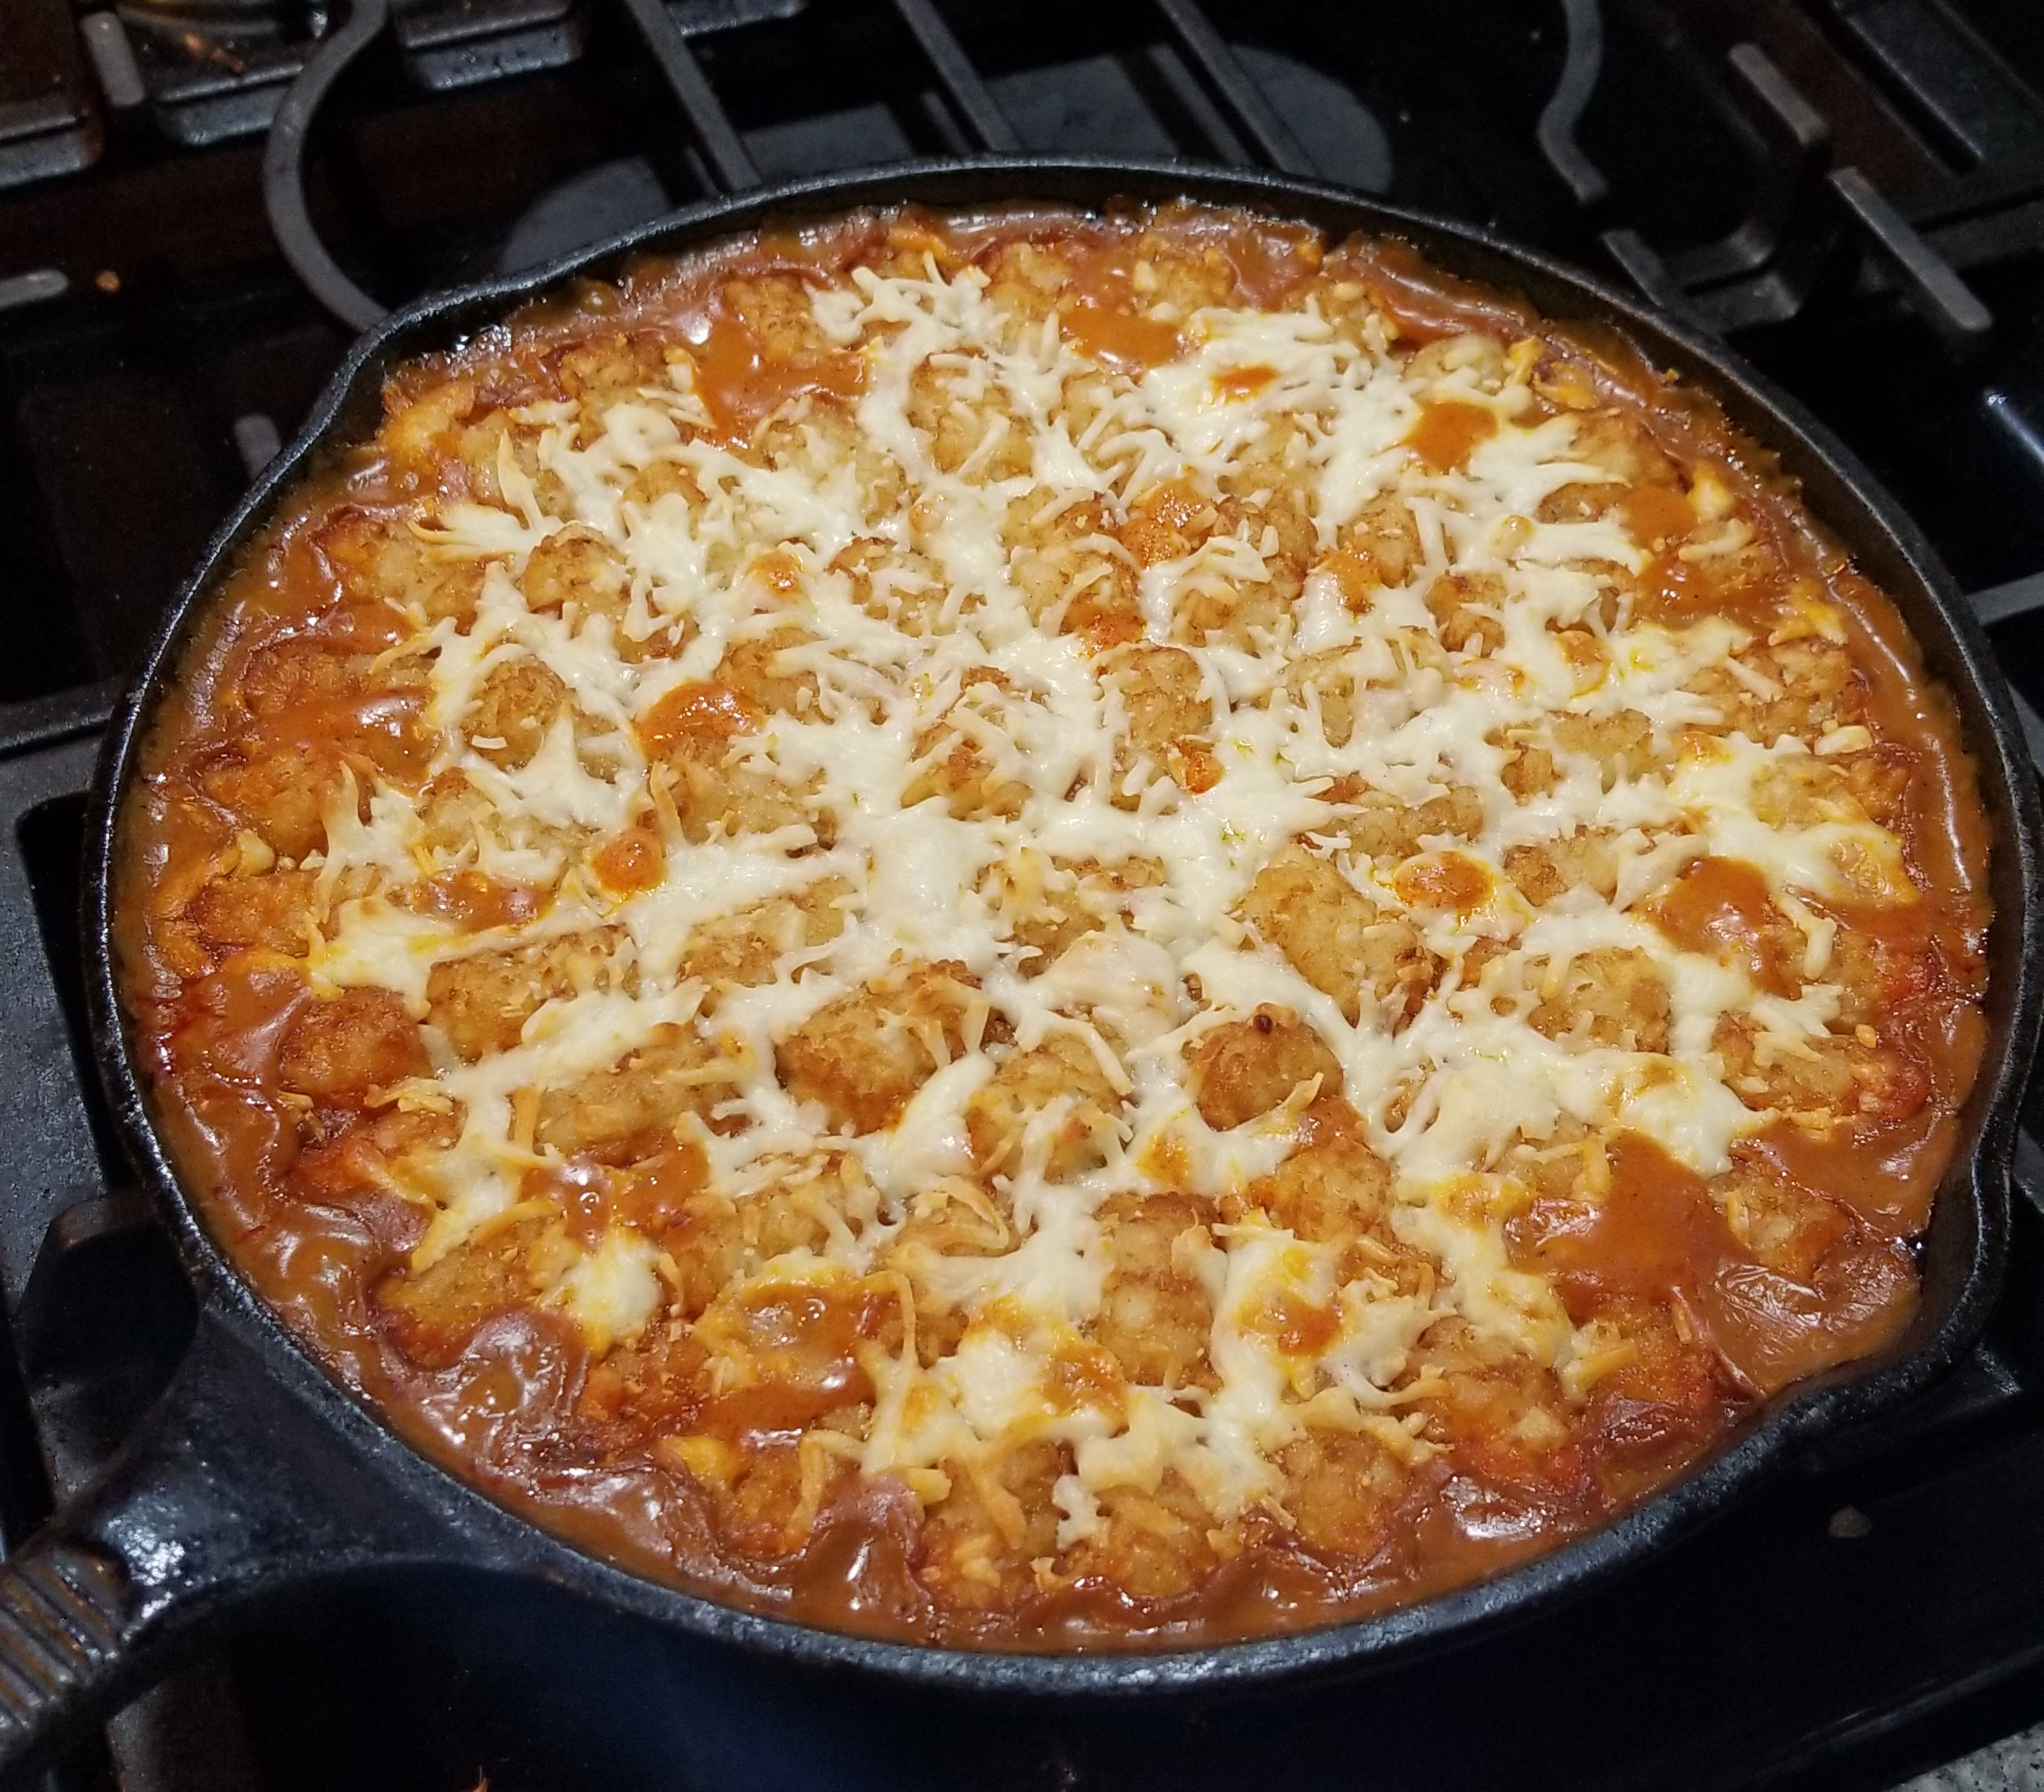
\includegraphics[width=.5\textwidth]{FoodPictures/tatertotcasserole.png}
	\end{figure}
\ingredients[13]{%
	\unit[\nicefrac{1}{2}]{large}& onion \\
	\unit[3]{cloves} & garlic \\
	\unit[6]{patties} & veggie sausage \\
	\unit[1]{can} & cream of mushroom soup \\
	\unit[16]{oz} & frozen veggies \\
	\unit[1]{tsp} & thyme \\
	\unit[1]{tsp} & paprika \\
	\unit[1]{tsp} & chili powder \\
	\unit[1]{tbsp} & flour \\
	\unit[1]{cups} & oat milk \\
	\unit[4]{cups} & tater tots \\
	\unit[1]{cup} & cheese(optional)\\
}
\preparation{%
	\step Preheat the oven to 350 \faren
	\step Heat about a tablespoon of oil in a 12-inch cast iron skillet on medium heat.
	\step Add the onions, cook for 2-3 minutes. Then add the garlic. Continue cooking until the onions are soft and starting to brown.
	\step Add the sausage patties (or other sausage) and stir for a couple of minutes until it starts to brown.
	\step Add the frozen veggies of your choice, mix, and let them cook for another 2-3 minutes.
	\step Add the cream of mushroom soup and mix well to combine.
	\step Add the spices, salt and pepper; thoroughly combine.
	\step Add 1 cup of oat milk and the flour, stir to combine. Then bring to a boil.
	\step Turn off the heat. Then layer the top of the mixture with frozen tater tots.
	\step Place into the oven and bake for 55 minutes.
	\step Remove from the oven and let sit for 5 minutes to cool.
}
\end{recipe}


\newpage
\section{Bread}
\begin{recipe}[preparationtime={\unit[2.5]{hours}},bakingtime={\unit[30-35]{minutes}},portion={2 loaves},source=\url{https://www.tasteofhome.com/recipes/basic-homemade-bread/}]{White Sandwich Bread}
\index{Bread}
\ingredients[8]{%
\unit[1]{cup} & water \\
\unit[2]{tsp} & active dry yeast \\
\unit[1]{cup} & milk \\
\unit[2]{tbsp} & butter \\
\unit[2]{tbsp} & sugar \\
\unit[1]{tbsp} & salt \\
\unit[715]{g} & all-purpose flour \\
& oil \\
}
\preparation{%
\step Mix the yeast, sugar and warm water(warm but should be able to keep a finger in it for a bit) in the bowl of the stand mixer. Let stand for about 5 minutes
\step Melt the butter and combine with the milk and salt. Add the mixture to the yeast mixture. Add 130 grams (1 cup) of the flour and mix until a clumpy mixture is formed.
\step Add the remaining 585 grams of flour to the stand mixture, gradually, mixing as you add. Mix unitl a shaggy, floury dough is formed.
\step Knead the dough for 8 to 10 minutes. Add flour if the dough is sticking to the sides of the bowl a tablespoon at a time. Dough should form a ball without sagging, and spring back when poked.
\step Grease a large bowl and transfer the dough to the greased bowl. Flip the dough ball so it is covered in oil. Cover and let rise in a warm place until doubled in size, about one hour.
\step Split the dough into two equal pieces and form each piece into a loose ball. Let rest for 10 minutes.
\step Grease 2 loaf pans. Smash a ball into a rectangle with the palms of your hand. Then fold the rectangle into overlapping thirds, pinch to close the sides and the ends. Fold in half by pressing down in the middle and bringing the sides together, pinch to close on the ends and side. Repeat for the second loaf.
\step Move the loaves to the loaf pans, by flipping them seam side down. Then let rest in a warm place until they start to dome over the sides of the pan, about an hour.
\step Heat the oven to 425 \faren. Slash the top of the loaves with a serated knife before you put them in the oven. When you add the loaves to the oven reduce the heat to 375\faren. Bake for 30 to 35 minutes. They should sound hollow when tapped.
\step Cool on a wire rack until completely cool before slicing.
}
\end{recipe}


\newpage
\begin{recipe}[preparationtime={\unit[2.5-4]{hrs}, depending on rise time},bakingtime={\unit[15]{min}},portion={8 4-5 inch buns},source=\url{https://smittenkitchen.com/2009/07/light-brioche-burger-buns/}]{Light Brioche Burger Buns}
\index{Bread}\index{Burger}
\ingredients[11]{
\unit[1]{cup} + \unit[1]{tbsp} & water \\
\unit[3]{tbsp} & warm milk \\
\unit[2]{tsp} & active dry yeast \\
\unit[2\nicefrac{1}{2}]{tbsp} & sugar \\
2 & eggs \\
\unit[3]{cups} & bread flour \\
\unit[\nicefrac{1}{3}]{cup} & all-purpose flour \\
\unit[1\nicefrac{1}{2}]{tsp} & salt\\
\unit[2\nicefrac{1}{2}]{tbsp} & unsalted butter, softened\\
& sesame seeds (optional)
}
\preparation{
\step In a measuring cup, combine 1 cup warm water, milk, yeast, and sugar. Let stand until foamy, about 5 minutes. Meanwhile, beat 1 egg.
\step In a large bowl, whisk the flours with salt. Add the butter, divided into small pieces, and rub into the flower between your fingers, making crumbs.
\step Stir in yeast mixture and beaten egg and knead until smooth and elastic, 8-10 minutes. The dough will be on the sticky side, so it can be a bit messy. Try and leave the dough tackier than you would a round loaf.
\step Shape dough into a ball and return it to the bowl. Cover the bowl with plastic wrap or a towel and let rise in a warm place until doubled, 1-2 hours.
\step Line a baking sheet with parchment paper or a silicone baking mat. Divide the dough into 8 equal parts. Gently roll each into a ball and arrange 2-3 inches apart on the baking sheet. Cover loosely with plastic wrap or towel and let buns rise in a warm place for 1-2 hours.
\step Set a large shallow pan of water on the oven floor. Preheat oven to 400\faren with rack in center. Beat remaining egg with 1 tbsp water and brush on top of buns. Sprinkle with sesame seeds.
\step Bake buns, turning sheet halfway through, for about 15 minutes, until tops are golden brown. Transfer to a rack to cool completely.
}
\end{recipe}


\newpage
\begin{recipe}[preparationtime={\unit[3-4]{hrs}, depending on rise time},bakingtime={\unit[16-18]{min}},portion={6 buns},source=\href{https://www.youtube.com/watch/?v=gTGSUYMu6Ns}{Joshua Weissman}]{Fancy Burger Buns}
\index{Burger}\index{Bread}
	\ingredients[12]{%
		\unit[4]{tbsp} & milk \\
		\unit[2]{tbsp} & water \\
		\unit[20]{g} & bread flour \\
		\unit[\nicefrac{1}{2}]{cup} & milk \\
		\unit[1]{tbsp} & instant yeast \\
		\unit[320]{g} & bread flour \\
		\unit[1]{tsp} & salt \\
		\unit[35]{g} & sugar \\
		1 & egg \\
		1 & egg yolk \\
		\unit[3]{tbsp} & softened butter \\
		1 & egg \\
		splash & milk \\
	}
	\preparation{
		\step Combine the milk, water and bread flour in a small saucepan on medium-high heat and mix constantly until it comes together, this should happen quickly. It will begin to resemble a thick paste and no longer very liquidy.
		\step Warm the larger portion of milk to about 95\faren and combine with the yeast and let sit for 5-8 minutes.
		\step Combine the flour, sugar, and salt in the bowl of the stand mixer and whisk to combine.
		\step Using the dough-hook on low speed, add the yeast mixture and mix until combined. Then add in the sticky paste and mix until combined.
		\step Add the full egg and egg yolk while mixing on low speed.
		\step Increase the mixer speed to medium-low, and mix until everything is thoroughly combined. Scrape down the sides of the bowl intermittently.
		\step Gradually add the softened butter.
		\step Continue mixing for 3-5 minutes or until the dough is smooth.
		\step Make the dough into a large ball and place into a covered, greased bowl for 1-1.5 hours, or until doubled in size.
		\step Punch down the dough, then on a floured work surface, evenly divide the dough into 6 pieces.
		\step For each piece of dough, fold in the edges to make a more round dough then flip it over and pull it toward you. Then turn 90 degrees and pull again, repeating until the dough is a nice ball.
		\step Place all of the dough balls onto a sheet pan, with at least two inches between each ball. Cover with another tray, and let rise until doubled, 1.5-2 hours.
		\step Make an eggwash with the remaining milk and egg, then brush the top of the buns.
		\step Bake them at 375\faren for 16-18 minutes. Then brush them with melted butter afterwards, letting them cool on a wire rack.
	}
\end{recipe}


\newpage
\begin{recipe}[preparationtime={\unit[20]{min}},bakingtime={\unit[20-25]{min}},portion={8 tortillas},source=\url{https://www.kingarthurflour.com/recipes/simple-tortillas-recipe}]{Flour Tortillas}
\index{Tortilla}\index{Mexican}\index{No Yeast}
\ingredients[9]{
\unit[2\nicefrac{1}{2}]{cups} (298g) & all-purpose flour \\
\unit[1]{tsp} & baking powder \\
\unit[\nicefrac{1}{2}]{tsp} & salt \\
\unit[\nicefrac{1}{4}]{cup of any} & lard (57g), butter (57g), shortening (48g), or vegetable oil (50g)\\
\unit[\nicefrac{3}{4}-1]{cup} & hot water
}
\preparation{
\step In a medium-sized bowl, whisk together the flour, baking powder, and salt.
\step Add the lard (or butter, or shortening; if you're using vegetable oil, add it in step 3). Use your fingers or a pastry blender to work the fat into the flour until it disappears. Coating most of the flour with fat inhibits gluten formation, making the tortillas easier to roll out.
\step Pour in the lesser amount of hot water (plus the oil, if you're using it), and stir briskly with a fork or whisk to bring the dough together into a shaggy mass. Stir in additional water as needed to bring the dough together.
\step Turn the dough out onto a lightly floured counter and knead briefly, just until the dough forms a ball. If the dough is very sticky, gradually add a bit more flour.
\step Divide the dough into 8 pieces. Round the pieces into balls, flatten slightly, and allow them to rest, covered, for about 30 minutes (see tips, below). If you wish, coat each ball lightly in oil before covering; this ensures the dough doesn't dry out (not necessary though).
\step While the dough rests, preheat an ungreased cast iron griddle or skillet over medium high heat, about 400\faren.
\step Working with one piece of dough at a time, roll into a round about 8" in diameter. Keep the remaining dough covered while you work. Fry the tortilla in the ungreased pan for about 30 seconds on each side, or until air bubble form and browning occurs on each side. Repeat with the remaining dough balls.
}
\hint{
Use just enough water to bring the dough together. Too much water and you'll end up with a sticky dough that is difficult to handle.
}

\end{recipe}


\newpage
\begin{recipe}[portion={\unit[12]{tortillas}},source=\url{https://www.isabeleats.com/3-ingredient-authentic-mexican-corn-tortillas/}]{Corn Tortillas}        
	\ingredients[]{%
		\unit[2]{cups} & masa harina \\
		\unit[\nicefrac{2}{3}]{tsp} & salt \\
		\unit[1\nicefrac{1}{2}]{cups} & hot water \\
		\unit[1]{tsp} & olive oil \\
	}
	\preparation{%
		\step Mix the masa harina and salt in a large bowl.
		\step Pour the water and oil into the bowl, and mix until combined. Then form into a ball with your hands. The dough should be firm and springy when touched, if the mixture is too dry add more water in small amounts until the dough is springy and holds together.
		\step Place the ball in a bowl and cover. Let rest for 20 minutes.
		\step Divide the dough into 12 equal pieces, rolling each one into a ball and placing back into the covered container.
		\step Preheat a griddle over medium-high heat.
		\step Cut a gallon-sized ziploc bag on the sides, so it can open fully. Then place a ball inside the two halves and press down with a small casserole dish. You want it to be about \nicefrac{1}{8} inch thick.
		\step Place the tortilla on the hot griddle and cook for 20 seconds. Flip it over and cook for 20 more seconds.
		\step Flip again and cook for 40 more seconds or until it begins to bubble/puff. Flip again and cook until brown marks form.
		\step Remove the cooked tortilla and place in a kitchen towel inside of a large closable container to keep it warm and moist.
		\step Repeat for the remaining 11 tortillas.
	}
\end{recipe}        


\newpage
\input{Bread/roti}

\newpage
\begin{recipe}[preparationtime={\unit[20]{min}},bakingtime={\unit[15]{min}},portion={6 paratha},source=\url{https://www.cookwithmanali.com/aloo-paratha/}]{Aloo Paratha}
\index{Indian}\index{Bread}\index{No Yeast}
\ingredients[17]{
2 & medium potatoes, boiled \\
\unit[\nicefrac{1}{4}]{tsp} & ajwain \\
1 & green chili, finely chopped \\
\unit[2]{tbsp} & finely chopped cilantro \\
\unit[\nicefrac{1}{4}]{tsp} & cumin powder \\
\unit[\nicefrac{1}{4}]{tsp} & garam masala \\
\unit[\nicefrac{1}{4}]{tsp} & amchur \\
\unit[\nicefrac{1}{8}-\nicefrac{1}{4}]{tsp} & chili powder (adjust to taste) \\
\unit[\nicefrac{3}{4}]{tsp} & salt (to taste) \\
\unit[3-4]{tsp} & oil or ghee (for cooking) \\
\textbf{Dough:} & \\
\unit[190]{g} & whole wheat flour \\
\unit[1]{tsp} & vegetable oil \\
\unit[\nicefrac{1}{4}]{tsp} & salt \\
& water}
\preparation{
\step Boil your potatoes if you haven't already. You can also do this in the Instant Pot on high for 8-10 minutes, depending on the size of your potatoes.
\step In a bowl mix together whole wheat flour (atta), oil and salt. Add water little by little and mix.
\step Knead to form a smooth and soft dough. Cover and let the dough rest for 15-20 minutes.
\step Divide the dough into 4-6 equal parts.
\step To make the filling, mash the boiled potatoes and transfer to a bowl.
\step Add chopped cilantro, salt, ajwain, chopped green chili, cumin powder, chat masala, garam masala powder, amchur and red chili powder.
\step Mix till everything is well combined. Adjust spice levels to taste if needed. The stuffing is now ready.
\step To make the paratha, take one of the dough balls and using your rolling pin roll it into a circle. Apply little oil (optional) all over the rolled dough.
\step Place 2-3 tablespoons of stuffing in the center. Don't overfill else it will be difficult to roll.
\step Bring all the edges together and pinch to seal the edges. Flatten the dough ball using your hands.
\step Now using your rolling pin, roll the dough to a circle of 7-8 inch diameter. The trick here is to apply equal pressure while rolling. If you do that, your paratha will turn round automatically.
\step Transfer the rolled paratha onto the hot tawa.
\step Cook the side for a minute or two and then flip over. Apply oil or ghee on the half-cooked side and flip again.
\step Now apply oil on the other side as well. Press with a spatula and cook the paratha till both sides have golden brown spots on them.
\step Repeat with the remaining dough balls.
}
\end{recipe}


\newpage
\begin{recipe}[preparationtime={\unit[15]{min}},portion={2 pizzas},source=\url{https://www.bonappetit.com/recipe/pizza-dough-2}]{Pizza Dough}
\index{Pizza}
\ingredients[6]{
\unit[\nicefrac{3}{4}]{cup} & warm water \\
\unit[2\nicefrac{1}{4}]{tsp} & dry active yeast \\
\unit[2]{cups} (260g) & all purpose flour \\
\unit[1]{tsp} & sugar\\
\unit[\nicefrac{3}{4}]{tsp} & salt\\
\unit[3]{tbsp} & vegetable oil
}
\preparation{
\step Pour 3/4 cup warm water into small bowl; stir in yeast. Let stand until yeast dissolves, about 5 minutes.
\step Mix 2 cups flour, sugar, and salt in mixer.
\step Add yeast mixture and 3 tablespoons oil; process until dough forms a sticky ball.
\step Transfer to lightly floured surface. Knead dough until smooth, adding more flour by tablespoonfuls if dough is very sticky, about 1 minute. You can also do this in the mixer.
\step Transfer to a bowl coated in oil; turn dough in bowl to coat with oil. Cover bowl and let dough rise in warm draft-free area until doubled in volume, about 1 hour.
\step Punch down dough. Roll out dough. Start in center of dough, working outward toward edges but not rolling over them.
}
\hint{
This recipe can be done a day ahead. Leave the dough in the fridge after kneading and take it out a couple of hours before to let rise before rolling out.
}

\end{recipe}


\newpage
\begin{recipe}[preparationtime={\unit[30]{min} + \unit[45]{min} rise},bakingtime={\unit[15]{min}},portion={16 breadsticks},source=\href{https://www.foodnetwork.com/recipes/food-network-kitchen/almost-famous-breadsticks-recipe-1972945}{`Almost-Famous Breadsticks' from Food Network Magazine}]{Simple Breadsticks}
\index{Bread}
\ingredients[10]{
\unit[\nicefrac{1}{4} + 1\nicefrac{1}{4}]{cup} & warm water \\
\unit[2\nicefrac{1}{4}]{tsp} & dry active yeast \\
\unit[4\nicefrac{1}{4}]{cups} (560g) & all purpose flour \\
\unit[2]{tbsp} & sugar\\
\unit[1]{tbsp} & salt\\
\unit[2]{tbsp} & unsalted butter, softened\\
\unit[3]{tbsp} & unsalted butter, melted\\
\unit[\nicefrac{1}{2}]{tsp} & kosher salt \\
\unit{pinch} & garlic powder \\
\unit{pinch} & dried oregano
}
\preparation{
\step Place 1/4 cup warm water in the bowl of a mixer; sprinkle in the yeast and set aside until foamy, about 5 minutes. 
\step Add the flour, butter, sugar, fine salt and 1\nicefrac{1}{4} cups plus 2 tablespoons warm water; mix with the paddle attachment until a slightly sticky dough forms, 5 minutes. 
\step Knead the dough by hand on a floured surface until very smooth and soft, 3 minutes.
\step Roll into a 2-foot-long log; cut into 16 1\nicefrac{1}{2}-inch-long pieces.
\step Knead each piece slightly and shape into a 7-inch-long breadstick; arrange 2 inches apart on a parchment-lined baking sheet. Cover with a cloth; let rise in a warm spot until almost doubled, about 45 minutes. 
\step Preheat the oven to 400 \faren. Make the topping: Brush the breadsticks with 1\nicefrac{1}{2} tablespoons of the butter and sprinkle with \nicefrac{1}{4} teaspoon kosher salt. 
\step Bake until lightly golden, about 15 minutes. Meanwhile, combine the remaining \nicefrac{1}{4} teaspoon salt with the garlic powder and oregano.
\step Brush the warm breadsticks with the remaining 1\nicefrac{1}{2} tablespoons melted butter and sprinkle with the flavored salt.
}

\end{recipe}


\newpage
\begin{recipe}[source=\href{http://jgradspittsburgh.com/about/}{JGrads Pittsburgh},portion={2 Large Loaves}]{Sweet Challah}
\index{Jewish}\index{Bread}
	\ingredients[8]{%
		\unit[1\nicefrac{1}{2}]{tbsp} & active dry yeast \\
		\unit[2\nicefrac{1}{2}]{cups} & water \\
		\unit[150]{g} & sugar \\
		\unit[\nicefrac{1}{2}]{tbsp} & salt \\
		1 & egg \\
		\unit[\nicefrac{1}{2}]{cups} & oil \\
		\unit[1,040]{g} & all-purpose flour \\
		1 & egg \\
		splash & milk \\
	}
	\preparation{%
		\step Warm the water to about 90-95\faren (warm to the touch but you should be able to keep your finger in it for a moment).
		\step Combine the yeast and the water in the bowl of a stand mixer; mix to combine. No need to let the yeas mixture rise.
		\step Add the sugar, salt, eggs and oil. Mix until well combined.
		\step Using the dough hook attachment to mix, gradually add the flour until the dough is thick and only a little sticky.
		\step Grease a large bowl with some additional oil, then add the dough to the bowl. Flip the dough so it is well covered in oil. Let rise for about 1 hour or until doubled in size.
		\step Remove from the bowl and knead the dough on a lightly-floured surface (adding some flour if needed) until the dough is soft and not very sticky. Separate into two equal pieces.
		\step Working with one of the pieces, divide into 3 equal pieces and roll into long logs. Combine the logs at one end and press together to remove the seams, then braid the 3 pieces until there is nothing left to braid. Combine and press again to prevent unfolding.
		\step Repeat for the second loaf, then let the loaves rest for about 30 minutes.
		\step Combine the last egg and milk and scramble together to make an egg wash.
		\step Preheat the oven to 350\faren.
		\step Use a pastry bush to coat the top of the loaves with egg wash. At this point you can add whatever additional toppings you would like.
		\step Bake for 30-35 minutes, switching racks halfway through.
		\step Let cool on a wire cooling rack.
	}
\end{recipe}


\newpage
\begin{recipe}[source=\href{https://cooking.nytimes.com/recipes/1016071-homemade-pita-bread}{New York Times Cooking}]{Pita}
	\index{Bread}\index{Mediterranean}\index{Israeli}	
	\ingredients[4]{%
		\unit[2]{tsp} & active dry yeast \\
		\unit[\nicefrac{1}{2}]{tsp} & sugar \\
		\unit[35]{g} & whole wheat flour \\
		\unit[260]{g} & all-purpose flour \\
		% Original recipe said to use 310 g and reserve 1/2 cup for dusting, so may need slightly more or less flour 
		\unit[1]{tsp} & kosher salt \\
		\unit[2]{tbsp} & olive oil \\
	}

	\preparation{%
		\step In a large bowl, combine the yeast and sugar with 1 cup of lukewarm water. Stir until well dissolved.
		\step Add the whole-wheat flour and about 40 grams of the all-purpose flour. Whisk everything together and place in a warm area, uncovered for about 15 minutes or until frothy and bubbling.
		\step Add the salt, olive oil, and the remaining all-purpose flour. Stir until the mixture forms a shaggy mass. Dust with a little bit of flour and knead in the bowl for 1 minute.
		\step Turn dough onto work surface and knead for about 2 minutes or until smooth. Cover and let rest for 10 minutes.
		\step Knead again for 2 minutes. Try not too add too much flour, the dough should be soft and a bit moist. (After this step you can put the dough into a container and refridgerate up-to overnight, making sure to bring back to room temperature before continuing)
		\step Put the dough in a clean bowl, cover, and let rest in a warm place until doubled in size (about 1 hour)
		\step Heat the oven to 475 \faren. Put a baking sheet (or large cast iron) on the bottom shelf to heat up.
		\step Punch down the dough and divide into 8 pieces. Form each piece into a small ball, cover the balls, and let rest for 10 minutes.
		\step Press a ball into a flat disk with a rolling pin. Then roll into a 6" circle, then into an 8" circle (about \nicefrac{1}{8}" thick)
		\step Place the dough onto the hot baking sheet and put back into the oven. After 2 minutes, flip the dough (it should be puffed). Bake for 1 more minute and transfer to a towel so that the bread stays soft.
		\step Repeat steps 9 and 10 for the remaining 7 pieces.
	}
            
\end{recipe}        


\newpage
\section{Dessert}
\begin{recipe}[source=\url{https://www.southernliving.com/recipes/fresh-peach-cobbler}]{Peach Cobbler}
\index{Cobbler}\index{Fruit}
\ingredients[9]{%
\unit[1/4]{cup} & butter \\
\unit[65]{g} & flour \\ 
\unit[200]{g} & sugar, divided \\
\unit[\nicefrac{1}{2}]{tbsp} & baking powder \\
\unit[1]{pinch} & salt \\
\unit[\nicefrac{1}{2}]{cup} & milk \\
\unit[2]{cups} & peach slices \\
\unit[\nicefrac{1}{2}]{tbsp} & lemon juice \\
\unit[1]{pinch} & ground cinnamon \\
\unit[1]{pinch} & ground nutmeg \\
}
\preparation{%
\step Preheat oven to 375 \faren. Add the butter to an 8x8 baking dish and put into oven to melt.
\step Combine the flour, 100 g of sugar, baking powder, and salt Add the milk and stir until the dry ingredients are moistened.
\step Bring the remaining sugar, peaches, and lemon juice up to a boil over high heat while stirring constantly.
\step Pour the batter over the melted butter, do not stir. Then pour the peach mixture over the batter, again without stirring. Sprinkle with cinnamon and nutmeg (optional)
\step Bake for 40 to 45 minutes.
}
\end{recipe}


\newpage
\begin{recipe}[source=\url{https://sallysbakingaddiction.com/super-moist-carrot-cake/}]{Carrot Cake}
\index{Cake}
\ingredients[20]{%
\unit[200]{g} & brown sugar \\
\unit[\nicefrac{3}{4}]{cup} & vegetable oil \\
\unit[60]{g} & greek yogurt \\
3 & eggs \\
\unit[2]{tsp} & vanilla extract \\
\unit[250]{g} & all-purpose flour \\
\unit[1]{tsp} & baking soda \\
\unit[2]{tsp} & ground cinnamon\\
\unit[\nicefrac{1}{4}]{tsp} & ground nutmeg \\
\unit[\nicefrac{1}{2}]{tsp} & salt \\
\unit[2]{cups} or \unit[260]{g} & finely grated carrots\\
\unit[\nicefrac{3}{4}]{cup} & pecan pieces\\
\\
\unit[8]{oz} (224g) & cream cheese, room temp\\
\unit[\nicefrac{1}{2}]{cup} (115g) & unsalted butter, softened\\
\unit[240-300]{g} & confectioners' suger\\
\unit[2]{tbsp} & heavy cream\\
\unit[2]{tsp} & vanilla extract\\
& salt to taste
}
\preparation{
\step Preheat oven to 350 \faren (177 \degree C). Spray 9 or 10inch springform pan with nonstick cooking spray.
\step Set out the cream cheese for the frosting so it may soften as you make the cake batter.
\step In a large bowl with a handheld or stand mixer fitted with a paddle attachment on medium speed, combine the brown sugar and oil. Beat in the yogurt until fully combined – about 60 seconds. Mixture will be gritty and thick. 
\step Add the eggs, one at a time, beating well after each addition. Mix in the vanilla. Set aside.
\step In a separate bowl, combine the flour, baking soda, cinnamon, nutmeg, and salt. 
\step With a spatula, manually stir the dry ingredients into the wet ingredients until just combined and all flour pockets are gone – do not overmix. Fold in the finely shredded carrots and pecan pieces. Pour or spoon batter into prepared springform pan.
\step Bake cake for 32-38 minutes or until toothpick inserted in the center comes out clean. Do not overbake, which will dry out cake. Check the cake at 30 minutes, then again at 32. Allow cake to cool completely before frosting.
\step To make the frosting, beat the softened cream cheese and butter together on medium speed for 2-3 minutes until soft, creamy, and combined thoroughly.
\step Add 2 cups of powdered sugar and beat until thick and combined. Add 2 Tablespoons heavy cream and 2 teaspoons vanilla extract. Beat on medium speed for 2 more minutes.
\step Add more powdered sugar until desired thickness is reached. Add salt to taste. 
}
\hint{
This recipe also can be made into 12 cupcakes. Bake time is 17-18 minutes.
}
\end{recipe}


\newpage
\begin{recipe}{Peanut Butter Cookies}
\index{Easy}
\ingredients[2]{
\unit[1]{cup} & sugar \\
\unit[1]{cup} & peanut butter \\
1 & egg \\
}
\preparation{
\step Preheat the oven to 350\faren
\step Cream together the peanut butter and sugar
\step Add the egg and mix until well combined. 
\step Portion onto a baking sheet into spoonfuls. Using a fork, press down on the cookies twice making a crosshatch.
\step Bake for about 8 minutes, let it rest on a rack for about 5-10 minutes.
}

\hint{
\begin{itemize}
    \item You can add chocolate chips or oats to make these even more delicious!
    \item You can also bake these in a cast iron pan. In this case, bake for about 10-12 minutes.
\end{itemize}}
\end{recipe}{}


\newpage
\begin{recipe}[preparationtime={\unit[15]{min}},bakingtime={\unit[30]{min}},source=\url{https://www.thekitchenismyplayground.com/2015/07/chocolate-crack-pie.html}]{Chocolate Crack Pie}
\index{Easy}\index{Pie}\index{Chocolate}
\ingredients[5]{%
\unit[4]{oz.} & dark chocolate \\
\unit[\nicefrac{1}{2}]{cup} & butter \\
\unit[1]{cup} & sugar \\
2 & eggs \\
1 & pie crust
}
\preparation{%
\step Preheat oven to 350\faren
\step Melt the butter and chocolate together over low heat in a small saucepan
\step Remove from heat once melted and well combined. Add the sugar to the mixture and mix well.
\step Let the mixture rest for about 3 minutes. Beat the eggs in a small bowl.
\step Add the chocolate mixture to the eggs and mix well. Transfer to pie crust.
\step Bake the pie in the oven for about 30 minutes. Let cool for about 1 hour.
}
\end{recipe}{}


\newpage
\begin{recipe}[preparationtime={\unit[10]{min}},bakingtime={\unit[20]{min}},source=\url{https://www.makingthymeforhealth.com/vegan-avocado-brownies/}]{Vegan Avocado Brownies}
\index{Brownie}\index{Vegan}\index{Chocolate}\index{Avocado}
\ingredients[]{
\nicefrac{1}{2} & medium ripe avocado \\
\unit[1]{cup} + \unit[2]{tbsp} & plant-based milk \\
\unit[\nicefrac{1}{4}]{cup} & maple syrup \\
\unit[\nicefrac{1}{2}]{cup} & sugar \\
\unit[1]{cup} & all-purpose flour \\
\unit[\nicefrac{1}{2}]{cup} & unsweetened cocoa powder \\
\unit[1]{tsp} & baking soda \\
\unit[\nicefrac{1}{2}]{tsp} & salt \\
\unit[\nicefrac{1}{2}]{cup} & chocolate chips
}
\preparation{
\step Preheat the oven to 350\faren. Lightly grease an 8x8" baking dish.
\step In a blender, combine the avocado, soymilk, maple syrup and sugar. Blend for about 15-20 seconds, until smooth.
\step In a large bowl, combine the flour, cocoa powder, baking soda, and salt then stir together. 
\step Pour the wet ingredients in the blender into the bowl with the dry. Stir until combined. Then add the chocolate chips and mix until they are evenly distributed.
\step Bake in the oven for 15-20 minutes, until set. You should be able to stick a fork in the center and have it come out clean.
\step Allow to cool for at least 15 minutes before serving.
}

\hint{
\begin{itemize}
    \item You can substitute the flour for whole-wheat flour if desired. 
    \item Feel free to add walnuts or any other type of nut else to this recipe!
\end{itemize}
}
\end{recipe}


\newpage
\begin{recipe}{Chickpea Cookie Dough}
\ingredients[]{%
\unit[250]{g} & cooked chickpeas \\
\unit[\nicefrac{1}{4}]{cup} & nut/seed butter \\
\unit[1]{tsp} & vanilla extract \\
\unit[\nicefrac{1}{4}]{cup} & Almond flour \\
\unit[2]{tbsp} & maple syrup \\
\unit[\nicefrac{1}{4}]{cup} & chocolate chips \\
\unit[\nicefrac{1}{2}]{tsp} & salt \\
}
\preparation{
\step Add everything to a food processor except for the chocolate chips, process until smooth
\step Add the chocolate chips and mix them in by hand.
\step Cool for at least 2 hours or so in the fridge, overnight is usually best
}
\end{recipe}


\newpage
\begin{recipe}[source={Mom},bakingtime={\unit[65]{min}},portion={\unit[1]{loaf}}]{Chocolate Chip Banana Bread}
	\ingredients[10]{%
		\unit[\nicefrac{1}{2}]{cup} & butter \\
		\unit[334]{g} & sugar \\
		2 & eggs \\
		\unit[\nicefrac{1}{4}]{tsp} & salt \\
		\unit[1\nicefrac{1}{2}]{tsp} & baking powder \\
		\unit[\nicefrac{1}{2}]{tsp} & baking soda \\
		\unit[\nicefrac{1}{4}]{cup} & sour cream \\
		2-3 & bananas \\
		\unit[260]{g} & flour \\
		\unit[1]{tsp} & vanilla extract \\
		\unit[1]{cup} & chocolate chips \\
	}
	\preparation{%
		\step In the bowl of a stand mixer, cream together the butter and sugar.
		\step Preheat the oven to 350\faren
		\step While the sugar and butter are creaming together, dissolve the baking powder and baking soda into the sour cream and let sit until it starts to fluff.
                \step After the butter and cream are creamed and the sour cream is fluffy, add the salt and eggs and mix until combined.
		\step Add the sour cream to the stand mixer once it has fluffed.
		\step Peel the bananas, slightly mash, then mix in with the contents of the stand mixer.
		\step Gradually add the flour to the bowl of the stand mixer while mixing.
		\step Add the vanilla extract and chocolate chips, mix until the chocolate chips are thoroughly mixed in.
		\step Pour the mixture into a bread loaf pan.
		\step Bake for 65 minutes.
		\step Remove from loaf pan once slightly cool, then move to a cooling rack. The bread tastes great fresh or can be frozen and reheated later.
	}
\end{recipe}


\newpage
\begin{recipe}[source=\url{https://www.deliciousmagazine.co.uk/recipes/the-best-sticky-toffee-pudding/},portion={\unit[8]{portions}},preparationtime={\unit[30]{min}},bakingtime={\unit[50]{min}}]{Sticky Toffee Pudding}
\ingredients[27]{
        \unit[160]{g} & whole dates, stoned and roughly chopped \\
        \unit[150]{ml} & boiling water \\
        \unit[1]{tsp} & vanilla extract \\
        \unit[90]{g} & unsalted butter, softened \\
        \unit[150]{g} & light muscovado (or light brown) sugar \\
        2 & large eggs \\
        \unit[2]{tbsp} & black treacle (or molasses) \\
        \unit[175]{g} & self-raising flour \\
        \unit[1]{tsp} & baking soda \\
        \unit[100]{ml} & whole milk \\
                       & \\
        \multicolumn{2}{l}{\large Toffee Sauce} \\[0.2cm]
        \unit[225]{g} & light muscovado (or light brown) sugar \\
        good slug & brandy or rum \\
        \unit[100]{g} & unsalted butter, softened \\
        \unit[275]{ml} & double (or heavy) cream \\
        \unit[1]{tbsp} & black treacle (or molasses)
}
\preparation{
        \step Put the dates in a mixing bowl with the water. Leave for 30 minutes until cool, then mash with a fork to a rough pulp. Stir through the vanilla and set aside. Butter a 8x8 dish and set aside. Heat the oven to 335\faren/fan 300\faren.
        \step While the dates are soaking, use an electric mixer or wooden spoon to beat the 90g butter and 150g sugar until light and creamy. Add the eggs one at a time, beating well before adding the next. Beat in the black treacle, then mix the flour with the bicarb and gently fold in one third using a metal spoon or balloon whisk. Fold in a third of the milk, then repeat until all the flour and milk are used up. Stir the soaked dates, with their liquid, into the batter – it may curdle, but don’t worry. Spoon into the prepared dish.
        \step Bake for 50 minutes or until the pudding is risen and firm, and a skewer pushed into the middle comes out clean (cover with foil after 40 minutes if the edges are browning too much). If the skewer comes out with what looks like uncooked mixture on it, it might be a piece of date. Taste it – if you can taste uncooked flour it will need longer.
        \step Meanwhile, make the toffee sauce. Put the 225g sugar, brandy, 100g butter and half the cream in a large, heavy-based pan and heat gently. When the sugar has dissolved, turn up the heat, stir in the treacle and bubble, stirring, for 2-3 minutes until the mix is a rich toffee colour. Take the pan off the heat and stir in the rest of the cream. Keep warm.
        \step Leave the pudding to cool for 20 minutes, then skewer it all over and pour over half the sauce. Leave for another 15 minutes, then serve drizzled with the rest of the sauce, with our toasted nut and demerara ice cream, if you like.
}
\hint{
        \begin{itemize}
                \item \unit[175]{g} self-raising flour = \unit[175]{g} all-purpose flour + \unit[2]{tsp} baking soda + \unit[1]{tsp} salt
                \item You can substitute any other milk for the whole milk.
        \end{itemize}
}
\end{recipe}


\newpage
\begin{recipe}        
	\index{Kosher!Passover}\index{Kosher!Milk}
	\ingredients[]{%
		\unit[1]{cup} & salted butter \\
		\unit[1]{cup} & dark brown sugar \\
		6 & matzos \\
		\unit[20]{oz} & semisweet chocolate chips \\
		\unit[\nicefrac{1}{2}]{cup} & pecans \\
	}

	\preparation{%
		\step Melt the butter in a saucepan, then add the brown sugar and stir until dissolved.
		\step Bring to a boil and reduce to a simmer until thickened, about 5 minutes.
		\step Preheat the oven to 325\faren.
		\step Spread the matzah out on a couple of baking sheets and pour the hot mixture on top of the matzah. Spread out the sugar mixture with a rubber spatula.
		\step Bake in the oven for about 20 minutes, or until the sugar mixture is bubbly and thick.
		\step Immediately cover with chocolate and place back in the oven to melt the chocolate. Spread the chocolate out with a rubber spatula.
		\step Put the matzah into the fridge to harden the chocolate.
		\step Once the chocolate is hardened, you can remove them from the baking sheets and store them in the freezer in a bag for as long as you would like (I don't think it can go bad in the freezer).
	}
\end{recipe}        


\newpage
\begin{recipe}[
	source=\url{https://www.justonecookbook.com/dorayaki-japanese-red-bean-pancake/}
	]
	{Dorayaki(Red-bean pancakes)}
	\index{Japanese}
    \ingredients{%
	    4 & eggs \\
	    \unit[137]{g} & sugar \\
	    \unit[2]{tbsp} & honey \\
	    \unit[160]{g} & all purpose flour \\
	    \unit[1]{tsp} & baking powder \\
	    \unit[1-2]{tbsp} & water \\
	    \unit[1]{tsp} & neutral oil \\
	    \unit[1.1]{lb} & red bean paste (anko)
    }

    \preparation{%
	    \step In a large bowl, combine eggs, sugar, and honey and whisk well until the mixture becomes fluffy.
	    \step Sift flour and baking powder into the bowl and mix all together. Keep in the fridge to rest for 15 minutes.
	    \step The batter should be slightly smoother now. Stir in 1 Tbsp of water. Depends on the size of eggs and how accurate your flour measurement is, the water amount may vary but it should be 1-2 Tbsp.
	    \step Heat a large non-stick frying pan over medium-low heat (in between 250 and 300 \faren). It's best to take your time and heat slowly. Dip a paper towel in vegetable oil and coat the bottom of the pan with the oil. Then remove the oil completely (that's the key for evenly golden brown dorayaki surface). With a ladle or a small measuring cup (I use a \nicefrac{1}{4} cup measuring cup), pour 3 Tbsp of the batter from 3" (8 cm) above the pan to create 3" (8 cm) diameter pancakes.

    }
\end{recipe}        


\newpage
\section{Fermentation}
\begin{recipe}[source=\url{https://www.youtube.com/watch?v=LqPko6a3Wh4}]{Ginger Beer}
\index{Drink}
\ingredients[1]{%
\unit[10]{cups} & water (divided) \\
\unit[255]{g} & sugar (divided) \\
\unit[120]{g} & ginger (divided) \\
}
\preparation{%

{\large Start Ginger Bug}
\begin{enumerate}
    \item Finely chop 22 grams of ginger.
    \item Combine 2 cups water, 28 g sugar, and the ginger to a large glass jar. Cover with a cheesecloth and leave it alone
\end{enumerate}{}
{\large Feeding Ginger Bug}
\begin{enumerate}
    \item Every 24 hours add 28 g sugar and 22 grams chopped ginger to the ginger bug. Continue for about 3 days, or until bubbly.
\end{enumerate}{}
{\large Making Ginger Beer}
\begin{enumerate}
    \item Add 2 quarts of water (8 cups), 180 grams sugar, and 54 grams shredded ginger to a large pot. 
    \item Bring to a boil, then let simmer for 7-8 minutes. Turn off heat and let cool all the way to room temperature (this will take a long time)
    \item Strain the boiled ginger liquid and press out all the juices from the ginger into a large bowl (get one with a spout). Add 110 grams of the strained ginger bug and the juice of 3 lemons.
    \item Add the mixture to bottles that can hold pressure (we don't want an explosion of glass shards), make sure to leave about 2 inches of head space.
    \item Every 24 hours burp the bottles so they don't explode. After 7 days, or whenever you are happy, you can store the bottles in the fridge (you don't have to burp them in the fridge).
\end{enumerate}{}
}
\suggestion{You can use the ginger bug to make any juice into a nice fizzy drink, though be careful on the portioning of the ginger bug (i.e. 2 cups of juice needs about 30 grams of ginger bug)}
\end{recipe}


\section{Instant Pot}
\subsection*{Basic recipes and Durations}
\begin{table}[H]
    \centering
    \begin{tabular}{c|c|c|c|c}
        Food Item & Food Amount & Water Amount & Pressure Duration (min) & Natural Release(min) \\ \hline
        Basmati Rice & \unit[1]{cup} & \unit[1]{cup} & 8 & 2\\ \hline
        Brown Rice & \unit[1]{cup} & \unit[1]{cup} & 15 & 5 \\ \hline
        Chickpeas & \unit[1]{lb.} & \unit[6]{cup} & 50 & 10 \\ \hline
        Black Beans & \unit[1]{lb.} & \unit[6]{cup} & 30 & 15 \\
    \end{tabular}
    \label{tab:InstantPot}
\end{table}

\newpage
\begin{recipe}[source=\url{https://www.simplyhappyfoodie.com/instant-pot-black-eyed-peas/}]{Black-Eyed Peas}
\ingredients[]{%
\unit[1]{tbsp} & olive oil \\
\unit[1]{small} & onion \\
1 & bell pepper \\
4-5 & mushrooms \\
\unit[\nicefrac{1}{2}]{tsp} & thyme \\
\unit[3]{tsp} & paprika \\
\unit[\nicefrac{1}{2}]{tsp} & black pepper \\
\unit[1]{tsp} & salt \\
\unit[4]{cloves} & garlic \\
3 & dried chilies \\
\unit[3\nicefrac{1}{2}]{cups} & vegetable broth \\
\unit[2]{tsp} & balsamic vinegar \\
\unit[250]{g} & black-eyed peas \\
}
\preparation{%
\step Turn the pressure cooker to the saute function and add the oil.
\step Dice the onion, bell pepper and mushrooms. When the pot is hot add them to the pot, stirring occasionally until the onions start to turn translucent.
\step Add the thyme, paprika, pepper, and salt. Stir.
\step Add the garlic and dried peppers. Cook for about 30 seconds, stirring frequently.
\step Add the broth, vinegar, and black-eyed peas to the pot. Stir well.
\step Place the lid on the pressure cooker and set to pressure cook for 17 minutes (when the cooking is done start making the rice).
\step Let naturally vent for 15 more minutes.
}
\end{recipe}


\newpage
\begin{recipe}[source=\url{https://recipes.instantpot.com/recipe/mashed-potatoes/}]{Mashed Potatoes}       
	\ingredients[6]{%
		    \unit[3]{lbs} & russet potatoes \\
		    \unit[3]{cloves} & garlic \\
		    \unit[1]{cup} & water \\
		    \unit[\nicefrac{1}{2}]{cup} & milk \\
		    \unit[3]{tbsp} & unsalted butter \\
		    \unit[1]{tsp} & salt \\
		      & black pepper \\
	    }

	    \preparation{%
		\step Quarter the potatoes (and peel if you don't like skin in your mashed potatoes). Smash and peel the garlic.
		\step Combine the potatoes, garlic and water in the instant pot. 
		\step Manual cook for 8 minutes and quick release the pressure afterwards.
		\step Drain the potatoes, making sure to retain some of the cooking liquid.
		\step Add the solids back to the instant pot bowl, then add the butter and milk. Mash the potatoes, adding the reserved cooking liquid a bit at a time until the proper consistency is reached.
		\step Season with the salt and pepper.
	    }
\end{recipe}        


\newpage
\begin{recipe}[source=\url{https://www.justonecookbook.com/pressure-cooker-anko-red-bean-paste/}]{Japanese Red Bean Paste (Anko)}
\ingredients[5]{%
\unit[250]{g} & azuki beans \\
\unit[1000]{ml} & water (1:4 bean:water) \\
\unit[250]{g} & sugar \\
\unit[\nicefrac{1}{8}]{tsp} & salt 
}
\preparation{%
        \step Put the 250 g azuki beans in a strainer and place it inside a large bowl. Rinse the azuki beans in running water until water is clear. Discard any pieces that are floating. Drain water.
        \step Transfer the beans to the Instant Pot and add 1000 ml of water to your pressure cooker. 
        \step Turn the Instant Pot on and cook with high pressure for 25 minutes. Naturally release the pressure for 15-20 minutes after cooking. 
        \step Scoop the foam on the surface and discard (if you prefer the more refined taste, optional). Pick one bean and mash it with your fingers. If it is mashed easily, it's done. 
        \step Drain the azuki beans through a fine sieve. 
        \step Put azuki beans back in the Instant pot and add the sugar. Press the `Saute' button and select the `Low' option.
        \step Let the sugar dissolve completely, stirring occasionally with a wooden spoon. Continue cooking until you can draw a line in the azuki bean mixture with the wooden spatula and see the bottom of the pot for 1 second. Then turn off the Instant Pot and take out the inner bowl from the Instant Pot and \textbf{let the mixture cool for 5-10 minutes}. The mixture will thicken more as it cools down. 
        \step Transfer the warm azuki beans into the food processor or blender. This may need to be done in batches (original recipe uses 14 cup food processor). Alternatively, you can use a very fine mesh strainer and press the mixture through with a wooden spoon.
        \step Run the food processor or blender until the mixture becomes smooth texture.
        \step Transfer to an airtight container. When it’s cooled and thickened more, it’s ready to use.
}
\hint{
        This can be kept in the freezer. For easier storage, divide into 100g portions.
}
\end{recipe}


\newpage
\section{Substitutes}
\begin{recipe}{Chia Seed Egg}
\index{Egg}\index{Vegan}\index{Vegetarian}
\ingredients[]{%
\unit[2]{tbsp}(\unit[2]{tsp}) & Chia Seeds (Ground)\\
\unit[3]{tbsp} & Boiling Water \\
}
\preparation{
\step Mix together the chia seeds and boiling water
\step Wait 5 minutes for the chia seeds to gel, then use as you would a normal egg (may need to wait for the "egg" to cool first)
}
\end{recipe}


\printindex

\end{document}
